\documentclass{ximera}

%\usepackage{todonotes}

\newcommand{\todo}{}

\usepackage{tkz-euclide}
\tikzset{>=stealth} %% cool arrow head
\tikzset{shorten <>/.style={ shorten >=#1, shorten <=#1 } } %% allows shorter vectors

\usepackage{tkz-tab}  %% sign charts
\usetikzlibrary{decorations.pathreplacing} 

\usetikzlibrary{backgrounds} %% for boxes around graphs
\usetikzlibrary{shapes,positioning}  %% Clouds and stars
\usetikzlibrary{matrix} %% for matrix
\usepgfplotslibrary{polar} %% for polar plots
\usetkzobj{all}
\usepackage[makeroom]{cancel} %% for strike outs
%\usepackage{mathtools} %% for pretty underbrace % Breaks Ximera
\usepackage{multicol}

\usepackage{polynom}



\usepackage[many]{tcolorbox}  %% for titled boxes
\newtcolorbox{xbox}[1]{%
    tikznode boxed title,
    enhanced,
    arc=0mm,
    interior style={white},
    attach boxed title to top center= {yshift=-\tcboxedtitleheight/2},
    fonttitle=\bfseries,
    colbacktitle=white,coltitle=black,
    boxed title style={size=normal,colframe=white,boxrule=0pt},
    title={#1}}


\usepackage{array}
\setlength{\extrarowheight}{+.1cm}   
\newdimen\digitwidth
\settowidth\digitwidth{9}
\def\divrule#1#2{
\noalign{\moveright#1\digitwidth
\vbox{\hrule width#2\digitwidth}}}





\newcommand{\RR}{\mathbb R}
\newcommand{\R}{\mathbb R}
\newcommand{\N}{\mathbb N}
\newcommand{\Z}{\mathbb Z}

%\renewcommand{\d}{\,d\!}
\renewcommand{\d}{\mathop{}\!d}
\newcommand{\dd}[2][]{\frac{\d #1}{\d #2}}
\newcommand{\pp}[2][]{\frac{\partial #1}{\partial #2}}
\renewcommand{\l}{\ell}
\newcommand{\ddx}{\frac{d}{\d x}}
\newcommand{\ddt}{\frac{d}{\d t}}

\newcommand{\zeroOverZero}{\ensuremath{\boldsymbol{\tfrac{0}{0}}}}
\newcommand{\inftyOverInfty}{\ensuremath{\boldsymbol{\tfrac{\infty}{\infty}}}}
\newcommand{\zeroOverInfty}{\ensuremath{\boldsymbol{\tfrac{0}{\infty}}}}
\newcommand{\zeroTimesInfty}{\ensuremath{\small\boldsymbol{0\cdot \infty}}}
\newcommand{\inftyMinusInfty}{\ensuremath{\small\boldsymbol{\infty - \infty}}}
\newcommand{\oneToInfty}{\ensuremath{\boldsymbol{1^\infty}}}
\newcommand{\zeroToZero}{\ensuremath{\boldsymbol{0^0}}}
\newcommand{\inftyToZero}{\ensuremath{\boldsymbol{\infty^0}}}



\newcommand{\numOverZero}{\ensuremath{\boldsymbol{\tfrac{\#}{0}}}}
\newcommand{\dfn}{\textbf}
%\newcommand{\unit}{\,\mathrm}
\newcommand{\unit}{\mathop{}\!\mathrm}
\newcommand{\eval}[1]{\bigg[ #1 \bigg]}
\newcommand{\seq}[1]{\left( #1 \right)}
\renewcommand{\epsilon}{\varepsilon}
\renewcommand{\iff}{\Leftrightarrow}

\DeclareMathOperator{\arccot}{arccot}
\DeclareMathOperator{\arcsec}{arcsec}
\DeclareMathOperator{\arccsc}{arccsc}
\DeclareMathOperator{\si}{Si}
\DeclareMathOperator{\proj}{proj}
\DeclareMathOperator{\scal}{scal}


\newcommand{\tightoverset}[2]{% for arrow vec
  \mathop{#2}\limits^{\vbox to -.5ex{\kern-0.75ex\hbox{$#1$}\vss}}}
\newcommand{\arrowvec}[1]{\tightoverset{\scriptstyle\rightharpoonup}{#1}}
\renewcommand{\vec}{\mathbf}
\newcommand{\veci}{\vec{i}}
\newcommand{\vecj}{\vec{j}}
\newcommand{\veck}{\vec{k}}
\newcommand{\vecl}{\boldsymbol{\l}}

\newcommand{\dotp}{\bullet}
\newcommand{\cross}{\boldsymbol\times}
\newcommand{\grad}{\boldsymbol\nabla}
\newcommand{\divergence}{\grad\dotp}
\newcommand{\curl}{\grad\cross}
%\DeclareMathOperator{\divergence}{divergence}
%\DeclareMathOperator{\curl}[1]{\grad\cross #1}


\colorlet{textColor}{black} 
\colorlet{background}{white}
\colorlet{penColor}{blue!50!black} % Color of a curve in a plot
\colorlet{penColor2}{red!50!black}% Color of a curve in a plot
\colorlet{penColor3}{red!50!blue} % Color of a curve in a plot
\colorlet{penColor4}{green!50!black} % Color of a curve in a plot
\colorlet{penColor5}{orange!80!black} % Color of a curve in a plot
\colorlet{fill1}{penColor!20} % Color of fill in a plot
\colorlet{fill2}{penColor2!20} % Color of fill in a plot
\colorlet{fillp}{fill1} % Color of positive area
\colorlet{filln}{penColor2!20} % Color of negative area
\colorlet{fill3}{penColor3!20} % Fill
\colorlet{fill4}{penColor4!20} % Fill
\colorlet{fill5}{penColor5!20} % Fill
\colorlet{gridColor}{gray!50} % Color of grid in a plot

\newcommand{\surfaceColor}{violet}
\newcommand{\surfaceColorTwo}{redyellow}
\newcommand{\sliceColor}{greenyellow}




\pgfmathdeclarefunction{gauss}{2}{% gives gaussian
  \pgfmathparse{1/(#2*sqrt(2*pi))*exp(-((x-#1)^2)/(2*#2^2))}%
}


%%%%%%%%%%%%%
%% Vectors
%%%%%%%%%%%%%

%% Simple horiz vectors
\renewcommand{\vector}[1]{\left\langle #1\right\rangle}


%% %% Complex Horiz Vectors with angle brackets
%% \makeatletter
%% \renewcommand{\vector}[2][ , ]{\left\langle%
%%   \def\nextitem{\def\nextitem{#1}}%
%%   \@for \el:=#2\do{\nextitem\el}\right\rangle%
%% }
%% \makeatother

%% %% Vertical Vectors
%% \def\vector#1{\begin{bmatrix}\vecListA#1,,\end{bmatrix}}
%% \def\vecListA#1,{\if,#1,\else #1\cr \expandafter \vecListA \fi}

%%%%%%%%%%%%%
%% End of vectors
%%%%%%%%%%%%%

%\newcommand{\fullwidth}{}
%\newcommand{\normalwidth}{}



%% makes a snazzy t-chart for evaluating functions
%\newenvironment{tchart}{\rowcolors{2}{}{background!90!textColor}\array}{\endarray}

%%This is to help with formatting on future title pages.
\newenvironment{sectionOutcomes}{}{} 



%% Flowchart stuff
%\tikzstyle{startstop} = [rectangle, rounded corners, minimum width=3cm, minimum height=1cm,text centered, draw=black]
%\tikzstyle{question} = [rectangle, minimum width=3cm, minimum height=1cm, text centered, draw=black]
%\tikzstyle{decision} = [trapezium, trapezium left angle=70, trapezium right angle=110, minimum width=3cm, minimum height=1cm, text centered, draw=black]
%\tikzstyle{question} = [rectangle, rounded corners, minimum width=3cm, minimum height=1cm,text centered, draw=black]
%\tikzstyle{process} = [rectangle, minimum width=3cm, minimum height=1cm, text centered, draw=black]
%\tikzstyle{decision} = [trapezium, trapezium left angle=70, trapezium right angle=110, minimum width=3cm, minimum height=1cm, text centered, draw=black]


\outcome{Determine how the graph of a function looks without using a calculator.}

% Synthesis of everything we've learned

% We've learned so much stuff!
% Can't we put this all together somehow?

% Let's make a concept map of everything we've learned so far.

% Holes, point discontinuities, review from limits at the beginning


\title[Break-Ground:]{What's the graph look like?}

\begin{document}
\begin{abstract}
Two young mathematicians discuss how to sketch the graphs of functions.
\end{abstract}
\maketitle

Check out this dialogue between two calculus students (based on a true
story):

\begin{dialogue}
\item[Devyn] Riley, I've been thinking about the derivative. 
\item[Riley] It's all about change. It's some ``change-detector'' tool
  for math.
\item[Devyn] I know!  What's crazy is that you can use it as a tool
  for sniffing out dirt on functions.
\item[Riley] First $f'$ tells us increasing or decreasing.
\item[Devyn] Then $f''$ tells us concavity.
\item[Riley] From just that we know all local maxes and mins.
\item[Devyn] And if we use limits, we can find any asymptotes!
\item[Riley] You know, I'd like to make up a procedure based on all
  these facts, that would tell me what the graph of any function would look like.
\item[Devyn] Me too! Let's get to work!
\end{dialogue}

\begin{problem}
  On some interval, we know that $f'(x)$ is positive and $f''(x)$ is positive.
  Which of the following is the best option for the shape of the graph on that
  interval?
  \begin{multipleChoice}%%BADBAD picture in the choices ok?
    \choice[correct]{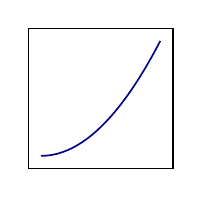
\begin{tikzpicture}[framed,scale=.5,baseline=3ex]
	\begin{axis}[
            clip=false,
            domain=0:1,
            ymax=1,
            height=4.5cm,
            ymin=0,
            axis lines=none,
          ]
          \addplot [very thick, penColor, smooth] {x^2};
        \end{axis}
        \end{tikzpicture}}
	\choice{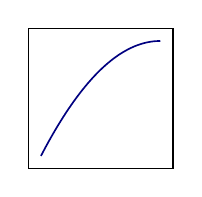
\begin{tikzpicture}[framed,scale=.5,baseline=3ex]
	\begin{axis}[
            clip=false,
            height=4.5cm,
            domain=0:1,
            ymax=1,
            ymin=0,
            axis lines=none,
          ]
          \addplot [very thick, penColor, smooth] {-(x-1)^2+1};
        \end{axis}
\end{tikzpicture}}
	\choice{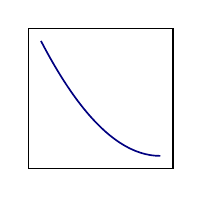
\begin{tikzpicture}[framed,scale=.5,baseline=3ex]
	\begin{axis}[
            clip=false,
            height=4.5cm,
            domain=0:1,
            ymax=1,
            ymin=0,
            axis lines=none,
          ]
          \addplot [very thick, penColor, smooth] {(x-1)^2};
        \end{axis}
\end{tikzpicture}}
	\choice{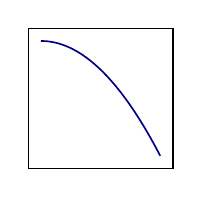
\begin{tikzpicture}[framed,scale=.5,baseline=3ex]
	\begin{axis}[
            clip=false,
            height=4.5cm,
            domain=0:1,
            ymax=1,
            ymin=0,
            axis lines=none,
          ]
          \addplot [very thick, penColor, smooth] {-x^2+1};
        \end{axis}
\end{tikzpicture}}
  \end{multipleChoice}
\end{problem}

\begin{problem}
  On some interval, we know that $f'(x)$ is negative and $f''(x)$ is positive.
  Which of the following is the best option for the shape of the graph on that
  interval?
  \begin{multipleChoice}%%BADBAD picture in the choices ok?
  	\choice{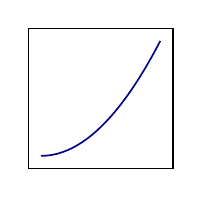
\begin{tikzpicture}[framed,scale=.5,baseline=3ex]
	\begin{axis}[
            clip=false,
            domain=0:1,
            ymax=1,
            height=4.5cm,
            ymin=0,
            axis lines=none,
          ]
          \addplot [very thick, penColor, smooth] {x^2};
        \end{axis}
        \end{tikzpicture}}
	\choice{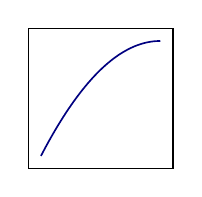
\begin{tikzpicture}[framed,scale=.5,baseline=3ex]
	\begin{axis}[
            clip=false,
            height=4.5cm,
            domain=0:1,
            ymax=1,
            ymin=0,
            axis lines=none,
          ]
          \addplot [very thick, penColor, smooth] {-(x-1)^2+1};
        \end{axis}
\end{tikzpicture}}
	\choice[correct]{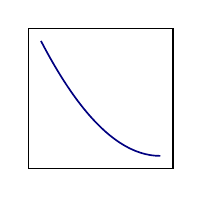
\begin{tikzpicture}[framed,scale=.5,baseline=3ex]
	\begin{axis}[
            clip=false,
            height=4.5cm,
            domain=0:1,
            ymax=1,
            ymin=0,
            axis lines=none,
          ]
          \addplot [very thick, penColor, smooth] {(x-1)^2};
        \end{axis}
\end{tikzpicture}}
	\choice{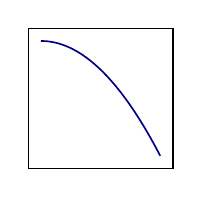
\begin{tikzpicture}[framed,scale=.5,baseline=3ex]
	\begin{axis}[
            clip=false,
            height=4.5cm,
            domain=0:1,
            ymax=1,
            ymin=0,
            axis lines=none,
          ]
          \addplot [very thick, penColor, smooth] {-x^2+1};
        \end{axis}
\end{tikzpicture}}
  \end{multipleChoice}
\end{problem}

%\input{../leveledQuestions.tex}
\end{document}
